\section{Results}
\label{sec:results}

\begin{table*}[t]
\centering
\caption{\textbf{Equal-budget comparison on RULER needle retrieval (16K characters).} Recall averaged over three NIAH tasks ($N{=}25$ each) per reader, at two rendering densities (uniform 5\,px $\approx$ 21 and 6\,px $\approx$ 14 characters per vision token). A, U, Z, and S are images with the same vision-token budget; \textbf{bold} marks the best among them. K adds anchors (verbatim text copies of the flagged strings) to A and is shown in gray because it spends extra text tokens. The last row is the provider-billed prompt-token count averaged over the readers that report usage. Hazard-aware rendering (S) is significantly worse than U or Z in none of the 72 paired comparisons (36 reader$\times$task$\times$density cells $\times$ 2 baselines) and significantly better in 63.}
\label{tab:baselines}
\small
\setlength{\tabcolsep}{4.2pt}
\begin{tabular}{l ccccc ccccc}
\toprule
& \multicolumn{5}{c}{5\,px budget ($\approx$21 chars/vtok)} & \multicolumn{5}{c}{6\,px budget ($\approx$14 chars/vtok)} \\
\cmidrule(lr){2-6}\cmidrule(lr){7-11}
Reader & A & U & Z & S (ours) & \textcolor{gray}{K} & A & U & Z & S (ours) & \textcolor{gray}{K} \\
\midrule
Claude Sonnet 5.5 & 0.14 & 0.22 & 0.19 & \textbf{0.79} & \textcolor{gray}{0.95} & 0.57 & 0.64 & 0.46 & \textbf{0.92} & \textcolor{gray}{1.00} \\
Gemini 3.5 Flash-Lite & 0.41 & 0.57 & 0.79 & \textbf{1.00} & \textcolor{gray}{1.00} & 0.88 & 0.78 & 0.84 & \textbf{1.00} & \textcolor{gray}{1.00} \\
GPT-6 Luna & 0.02 & 0.03 & 0.02 & \textbf{0.50} & \textcolor{gray}{0.91} & 0.11 & 0.16 & 0.08 & \textbf{0.65} & \textcolor{gray}{0.82} \\
Qwen3-VL-235B & 0.00 & 0.00 & 0.00 & \textbf{0.55} & \textcolor{gray}{1.00} & 0.07 & 0.08 & 0.03 & \textbf{0.60} & \textcolor{gray}{1.00} \\
Llama 4 Maverick & 0.00 & 0.00 & 0.00 & \textbf{0.58} & \textcolor{gray}{0.97} & 0.00 & 0.01 & 0.00 & \textbf{0.59} & \textcolor{gray}{0.90} \\
MiniMax-M3 & 0.00 & 0.00 & 0.00 & \textbf{0.57} & \textcolor{gray}{1.00} & 0.02 & 0.01 & 0.00 & \textbf{0.42} & \textcolor{gray}{0.97} \\
\midrule
\textit{Mean} & 0.09 & 0.14 & 0.17 & \textbf{0.66} & \textcolor{gray}{0.97} & 0.28 & 0.28 & 0.23 & \textbf{0.70} & \textcolor{gray}{0.95} \\
\textit{Billed tokens} & 779 & 775 & 768 & 779 & \textcolor{gray}{823} & 913 & 891 & 887 & 812 & \textcolor{gray}{960} \\
\bottomrule
\end{tabular}
\end{table*}


\subsection{Equal-budget comparison}
\label{sec:main}

\Cref{tab:baselines} compares all image arms at the same vision-token budget on 16K-character RULER documents.
Averaged over five readers, uniform rendering recovers 8\% of needles at the denser budget and 22\% at the lighter one.
Claude Sonnet 5.5 (0.57) and Gemini (0.88) are the only readers above 0.11 at 6\,px.
Allocation (S) raises the mean to 0.64 and 0.65, a pooled gain of 0.55 and 0.43 whose confidence intervals exclude zero by a wide margin (\cref{tab:pooled}).
After Holm correction, the gain is significant in 14 and 11 of 15 cells and never significantly negative.
The two stronger uniform baselines barely help: font/size search (U) reaches 0.12 and 0.21, and render-then-downsample (Z) 0.16 and 0.19.
Both plausibly fall short because they spread legibility evenly over all characters.
At 6\,px, S is also 8\% cheaper than uniform rendering (842 vs.\ 920 billed tokens), because prose shrinks more than the enlarged strings grow.
The weaker readers gain most (at 6\,px Llama 4 Maverick from 0.00 to 0.59, GPT from 0.11 to 0.65), while Gemini, already at 0.88, gains 0.12.
Under the precision-aware F1, which penalizes returning several candidate values, the gains are smaller (0.46 and 0.34 pooled) but remain significant in at least 9 of 15 cells.

\paragraph{Targeting, enlargement, or salience?}
Two controls separate the ingredients of S.
Arm R runs the same allocation on randomly chosen ordinary words, matched in total length, so its sizes and cost are close to those of S while the needles shrink with the prose.
R recovers 0.10 of the needles at both budgets, and S exceeds it by 0.54 and 0.56.
Arm B keeps every glyph at the uniform size but draws a box around each flagged string, which makes the needle easy to \emph{find} but not easier to \emph{read}.
B is 0.53 below S and slightly worse than uniform rendering ($-$0.05, CI upper bound $-$0.001; \cref{tab:pooled}), perhaps because the box line touches the small glyphs.
The gain therefore comes from making the targeted strings legible, not from layout changes or from pointing at the needle.

\begin{table}[t]
\centering
\caption{\textbf{Pooled effects} over the five non-Claude readers (recall unless noted). CI: 95\% bootstrap over readers and items. Sig.: cells (reader $\times$ task) significantly positive after Holm correction within each row; neg.: significantly negative.}
\label{tab:pooled}
\footnotesize
\setlength{\tabcolsep}{2.5pt}
\begin{adjustbox}{max width=\columnwidth}
\begin{tabular}{l c c c c}
\toprule
Comparison & $\Delta$ & 95\% CI & sig. & neg. \\
\midrule
\multicolumn{5}{l}{\textit{Equal budget, RULER}} \\
\name $-$ COC, 16K, 5\,px & +0.55 & [+0.48, +0.62] & 14/15 & 0 \\
\name $-$ COC, 16K, 6\,px & +0.43 & [+0.27, +0.56] & 11/15 & 0 \\
\name $-$ COC, 32K--128K, 6\,px & +0.48 & [+0.43, +0.53] & 35/45 & 0 \\
\name $-$ font search, 6\,px & +0.44 & [+0.31, +0.55] & 11/15 & 0 \\
\name $-$ random words, 6\,px & +0.56 & [+0.47, +0.64] & 12/15 & 0 \\
box $-$ COC, 6\,px & -0.05 & [-0.13, 0.00] & 0/15 & 1 \\
\name $-$ box, 6\,px & +0.53 & [+0.41, +0.64] & 14/15 & 0 \\
half $-$ COC, 5\,px & +0.30 & [+0.21, +0.40] & 9/10 & 0 \\
half $-$ COC, 6\,px & +0.21 & [0.00, +0.39] & 8/10 & 0 \\
\name $-$ half, 6\,px & +0.31 & [+0.20, +0.41] & 6/10 & 0 \\
\midrule \multicolumn{5}{l}{\textit{Milder budgets (32K)}} \\
\name $-$ COC, 10\,px & +0.20 & [+0.11, +0.30] & 4/10 & 0 \\
\name $-$ font search, 10\,px & +0.04 & [-0.04, +0.12] & 1/10 & 1 \\
\midrule \multicolumn{5}{l}{\textit{Natural strings (LongBench documents)}} \\
\name $-$ COC, flagged targets & +0.25 & [+0.12, +0.38] & 4/5 & 0 \\
\name $-$ COC, detector-indep. & -0.01 & [-0.11, +0.08] & 0/5 & 0 \\
\midrule \multicolumn{5}{l}{\textit{Ordinary comprehension (LongBench F1)}} \\
\name $-$ COC & +0.02 & [-0.02, +0.06] & 0/10 & 0 \\
\name+anchor $-$ text & -0.21 & [-0.29, -0.13] & 0/10 & 9 \\
\midrule \multicolumn{5}{l}{\textit{Post-processing: {\name}+anchor $-$ COC+anchor (all settings: \cref{tab:app_pooled,tab:app_pooled2})}} \\
RULER 16K, 6\,px (F1) & +0.04 & [0.00, +0.08] & 1/15 & 0 \\
multi-key 64K--128K (F1) & -0.01 & [-0.05, +0.03] & 0/10 & 0 \\
natural, flagged, 6\,px & +0.02 & [-0.06, +0.10] & 0/5 & 0 \\
\bottomrule
\end{tabular}
\end{adjustbox}
\end{table}


\subsection{Why does allocation work?}
\label{sec:why}

\begin{figure}[t]
\centering
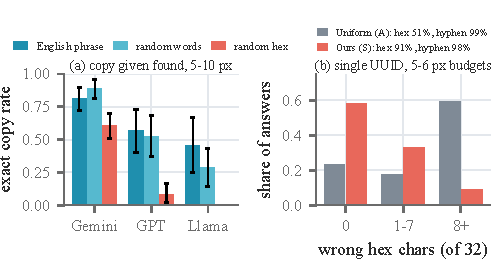
\includegraphics[width=\columnwidth]{fig/why.pdf}
\caption{\textbf{Reading is limited by what the language prior cannot supply.} (a) Controlled study: 32-character targets of three types hidden in the same 16K-character documents and rendered uniformly at 5--10\,px. Among answers in which the reader found the target, the share copied exactly (95\% CI), for the three readers that found enough targets of every type. (b) Single-UUID needles at the 5 and 6\,px budgets: wrong hexadecimal characters per answer of the right length. Under uniform rendering most such answers are fabricated, and under allocation most are exact.}
\label{fig:why}
\end{figure}

\Cref{sec:principle} predicts that readers fail where the pixels must supply what the language prior cannot.
Three observations on the single-UUID needles of \cref{tab:baselines} (five readers, both budgets, and the box runs) are consistent with this.

\emph{The format is read, the content is not.}
Under uniform rendering, a third of the answers are empty.
In the answers of the right length, the four hyphens, which the UUID format predicts, are correct 99\% of the time, but the 32 hexadecimal characters only 51\% of the time.
Allocation raises the hexadecimal characters to 91\% and leaves the hyphens at 98\%. The gain holds for every reader (from 0.15--0.96 to 0.82--1.00).

\emph{Wrong answers are fabricated, not misread.}
If uniform rendering merely blurred a few glyphs, errors would be spread over a few characters.
Instead, 59\% of the right-length answers have at least 8 of 32 characters wrong, with a median of 27, close to the 30 expected from guessing (\cref{fig:why}b). Only 23\% are exact.
The weaker readers drive this pooled pattern. All right-length answers of Llama and MiniMax, and most of those of Qwen and GPT, reproduce the format and invent the content, consistent with \cref{eq:reading}. Gemini, the strongest reader, almost never fabricates and errs by misreading (\cref{app:why}).
Under allocation, 58\% of the answers are exact and 9\% are fabricated.
Among partial misreads under uniform rendering, the most frequent confusion is 8$\to$0 (24 of 89 wrong characters). The two glyphs differ by a small stroke, which a patch holding three or four characters blurs.

\emph{The pixels needed depend on predictability.}
To test this, we hid one 32-character value in the same RULER documents (16K characters) and varied only its type: an English phrase from LongBench passages, random common words, or random hexadecimal characters.
Each document was rendered uniformly at 4--10\,px. We scored the answers in which the reader found the target (at least 50\% similar to it), which separates transcription from search (\cref{app:why}).
MiniMax and Qwen3-VL rarely found English or word targets and usually answered with the key instead, so we compare transcription for the three readers that found enough targets of every type.
For each of them, a found hexadecimal string is copied exactly far less often than a found English phrase at 5--10\,px: 0.61 vs.\ 0.82 for Gemini, 0.08 vs.\ 0.57 for GPT, and 0.00 vs.\ 0.46 for Llama (\cref{fig:why}a). Random words reach 0.89, 0.53, and 0.29.
Hexadecimal and English targets also differ in their glyphs, so this test supports but does not isolate the role of the prior (\cref{app:why}).

The account is also consistent with the boundaries of \cref{tab:pooled}: boxing does not help, suggesting legibility rather than search alone is the bottleneck; at 10\,px font/size search recovers most of the gain (S$-$U $+$0.04); dense hazards leave too few pixels to lift any string (\cref{app:density}); and shrinking prose costs little (\cref{sec:longbench}).

\subsection{Scaling with context length}
\label{sec:length}

\begin{figure}[t]
\centering
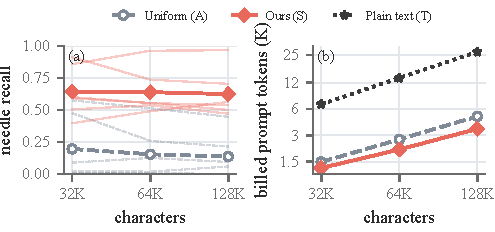
\includegraphics[width=\columnwidth]{fig/scaling.pdf}
\caption{\textbf{Context length.} RULER at 32K--128K characters (6\,px budget, up to three image pages, $N{=}20$ per task). (a) Needle recall; thin lines are individual readers (including Claude), thick lines the mean over five readers. (b) Billed prompt tokens averaged over the four of these readers that report usage; log scale.}
\label{fig:scaling}
\end{figure}

Optical compression is most attractive for long documents, so \cref{fig:scaling} extends the comparison to 128K characters.
Under uniform rendering, mean recall declines from 0.12 at 32K to 0.08 at 64K and 0.07 at 128K, consistent with reports that compressed reading loses retrieval ability as context grows~\cite{zhao2025vtcbench}.
Allocation stays between 0.60 and 0.56, a pooled gain of 0.48 [0.43, 0.53] with 35 of 45 cells significant after Holm correction.
It also uses 13\%, 23\%, and 27\% fewer billed tokens than uniform rendering at the three lengths.
On the four readers with billed costs for both, it uses 5.4$\times$, 6.8$\times$, and 8.0$\times$ fewer than plain text, which every reader answers with recall of at least 0.99.
Individual readers differ widely (0.47 to 0.97 at 128K for S; \cref{tab:app_length}).

\subsection{Milder budgets}
\label{sec:regime}

Our main budgets put most readers near the floor of uniform rendering, where gains are easiest to obtain.
We therefore repeated the single and multi-key tasks at 32K characters with base sizes of 8 and 10\,px, which cost 1.5 and 2.3 times as many vision tokens as 6\,px.
Uniform rendering improves with size (multi-key: 0.26 at 8\,px, 0.60 at 10\,px), and the gain of S shrinks accordingly, to 0.38 at 8\,px and 0.20 at 10\,px (\cref{tab:pooled}).
The font/size search catches up: S beats U by 0.26 at 8\,px but only by 0.04 at 10\,px, which is not significant.
Single UUIDs remain hard even here (A 0.20, S 0.44 at 10\,px).
Allocation is most useful where the budget is tight, which is also where optical compression saves the most.

\subsection{Naturally occurring strings}
\label{sec:niq}


RULER needles are synthetic, and our detector was designed with such strings in mind.
We built two sets of 60 questions from LongBench documents of up to 40K characters (ten each from six tasks).
Each asks for the exact string that follows a unique six-word phrase (\cref{app:niq}).
In the first set, targets are strings the detector flags, such as report and grant numbers, ISBNs, citation keys, and URLs.
Here allocation doubles mean recall (0.23 to 0.48, significant for four of five readers) at 12\% fewer billed tokens than uniform rendering (\cref{tab:niq}).
In the second set, targets are any digit-bearing tokens of at least four characters, sampled without the detector.
The detector flags only one of the 60, because most are short numbers, percentages, and version strings such as ``25,000'' or ``2.0.13''.
On these, every image arm is poor (0.36--0.45 against 0.96 for text), and allocation neither helps nor hurts ($-$0.01 [$-$0.11, 0.08]).
Shrinking prose to make room for flagged strings thus did not measurably damage the strings the detector misses, but nothing in the image protects them either.
A synthetic detector ablation agrees: needles the regex misses leave S at uniform recall (0.33 vs.\ 0.32), while an oracle detector would reach 0.82 (\cref{tab:detector}).

\subsection{Anchors on the allocated image}
\label{sec:anchors}

Anchors~\cite{anon2026renderretain} copy the flagged strings into the prompt.
In the essay haystacks of \cref{tab:baselines}, the only flagged strings are the needles. The anchor list \emph{is} then the answer, and K and X reach 0.90--1.00 by copying. On multi-key, readers often return the whole list (F1 0.46--0.52; \cref{app:rescore}).
We therefore compare K and X on the flagged natural identifiers, where documents carry 5.3 distinct anchors and a random pick would score 0.44.
Across base sizes of 5, 6, and 7\,px, X reaches 0.75--0.81 and lies on or above K's recall--cost frontier by 0.02--0.05, though no pooled interval excludes zero (\cref{app:anchors}).
At 64K--128K characters, X costs 29--31\% less than K, but under F1 the anchors add nothing over allocation alone.
When the target is not flagged, anchors can mislead (X 0.36 vs.\ 0.44 for S and K on the detector-independent set).
Beyond about 16 flagged strings per 32K characters, anchors on either image become expensive and ineffective, and routing to text~\cite{anon2026renderretain} takes over. On real corpora, prose goes to images and code and logs to text (\cref{app:density,app:corpora}).

\subsection{Effect on ordinary comprehension}
\label{sec:longbench}


Shrinking prose could hurt questions unrelated to identifiers.
On held-out LongBench documents of up to 40K characters (\cref{tab:longbench}), pooled F1 changes by +0.02 [$-$0.02, 0.06] for S and +0.02 [$-$0.03, 0.07] for X relative to uniform rendering, which rules out losses larger than about 0.03 (\cref{tab:pooled,tab:app_pooled2}). One reader--task cell is significantly negative for S, and none for X.
Relative to plain text, however, every image arm loses: X trails it by 0.15--0.33 F1 in 9 of 10 cells, at a fifth to a quarter of the text cost.
Allocation thus removes a failure specific to identifiers but does not make optical compression a substitute for text.

